\documentclass[12pt]{article}
\usepackage{fancyhdr}
\usepackage{amsmath,amsfonts,enumerate}
\usepackage{color,graphicx}
\usepackage{tikz}
\usepackage{pgfplots}
\usepackage{listings}
\usepackage{algorithm}
\usepackage{algorithmic}
\usetikzlibrary{arrows,positioning,shapes,calc,matrix}
\pagestyle{fancy}
%%%%%%%%%%%%%%%%%%%%%%%%%%%%%%%%%%%%%%%%%%%%%%%%%
% Course customization based on university sources
%%%%%%%%%%%%%%%%%%%%%%%%%%%%%%%%%%%%%%%%%%%%%%%%%
\newcommand{\masunitnumber}{CENG 403}
\newcommand{\examdate}{January 2025}
\newcommand{\academicyear}{2024-2025}
\newcommand{\semester}{I}
\newcommand{\coursename}{Deep Learning - CNN Visualization \& Classic Architectures (University Sources)}
\newcommand{\numberofhours}{3}
%%%%%%%%%%%%%%%%%%%%%%%%%%%%%%%%%%%%%%%%%%%%%%%%%
% CUSTOM SPACING COMMANDS FOR ANSWER SPACES
%%%%%%%%%%%%%%%%%%%%%%%%%%%%%%%%%%%%%%%%%%%%%%%%%
\newcommand{\answerspace}[1]{\vspace{#1}}
\newcommand{\questionspace}{\vspace{3cm}}        
\newcommand{\subquestionspace}{\vspace{2.5cm}}   
\newcommand{\shortanswer}{\vspace{2cm}}          
\newcommand{\mediumanswer}{\vspace{3cm}}         
\newcommand{\longanswer}{\vspace{4cm}}           
\newcommand{\journalspace}{\vspace{4.5cm}}       
\newcommand{\codespace}{\vspace{5cm}}            
%%%%%%%%%%%%%%%%%%%%%%%%%%%%%%%%%%%%%%%%%%%%%%%%%
% Header setup
%%%%%%%%%%%%%%%%%%%%%%%%%%%%%%%%%%%%%%%%%%%%%%%%%
\lhead{}
\rhead{}
\chead{{\bf MIDDLE EAST TECHNICAL UNIVERSITY}}
\lfoot{}
\rfoot{}
\cfoot{}
\begin{document}
\setlength{\headsep}{5truemm}
\setlength{\headheight}{14.5truemm}
\setlength{\voffset}{-0.45truein}
\renewcommand{\headrulewidth}{0.0pt}
\begin{center}
SEMESTER \semester\ EXAMINATION \academicyear
\end{center}
\begin{center}
{\bf \masunitnumber\ -- \coursename}
\end{center}
\vspace{20truemm}
\noindent \examdate\hspace{45truemm} TIME ALLOWED: \numberofhours\ HOURS
\vspace{19truemm}
\hrule
\vspace{19truemm}
\noindent\underline{INSTRUCTIONS TO CANDIDATES}
\vspace{8truemm}
%%%%%%%%%%%%%%%%%%%%%%%%%%%%%%%%%%%%%%%%%%%%%%%%%%%%%%
% Instructions based on university standards
%%%%%%%%%%%%%%%%%%%%%%%%%%%%%%%%%%%%%%%%%%%%%%%%%%%%%%
\begin{enumerate}
\item This examination paper contains {\bf SEVEN (7)} questions and comprises 
{\bf TEN (10)} printed pages.
\item Answer all questions. 
The marks for each question are indicated at the beginning of each question.
\item Answer each question beginning on a {\bf FRESH} page of the answer book.
\item This {\bf IS NOT an OPEN BOOK} exam.
\item Show all mathematical derivations clearly with proper notation.
\item For architectural diagrams, draw clear and labeled components.
\item Calculate all requested parameters and show intermediate steps.
\item Explain computational complexity where requested.
\end{enumerate}
%%%%%%%%%%%%%%%%%%%%%%%%%%%%%%%%%%%%%%%%%%%%%%%%%
% New page for questions
%%%%%%%%%%%%%%%%%%%%%%%%%%%%%%%%%%%%%%%%%%%%%%%%%
\newpage
\lhead{}
\rhead{\masunitnumber}
\chead{}
\lfoot{}
\cfoot{\thepage}
\rfoot{}
\setlength{\footskip}{45pt}
%%%%%%%%%%%%%%%%%%%%%%%%%%%%%%%%%%%%%%%%%%%%%%%%%%
% EXAM QUESTIONS BASED ON UNIVERSITY SOURCES
%%%%%%%%%%%%%%%%%%%%%%%%%%%%%%%%%%%%%%%%%%%%%%%%%%

\paragraph{Question 1. CNN Visualization Techniques and CAM Variants}{\hfill (25 marks)}\\
Based on Stanford CS231n and university computer vision course materials.

\begin{enumerate}[(a)]
    \item Implement Class Activation Mapping (CAM) for a CNN with Global Average Pooling. Given a feature map $F_k$ of size $H \times W$ for the $k$-th channel and weight $w_k$ connecting to class $c$: \hfill (10 marks)
    \begin{itemize}
        \item Derive the mathematical formulation for CAM: $M_c(x,y) = \sum_k w_k \cdot F_k(x,y)$
        \item Explain why CAM requires Global Average Pooling (GAP) layer
        \item Calculate the computational complexity for generating CAM for a 512×512 image with 512 feature maps
    \end{itemize}
    
    \journalspace
    
    \item Compare CAM with Grad-CAM and Grad-CAM++. Explain the following improvements: \hfill (10 marks)
    \begin{itemize}
        \item How Grad-CAM generalizes CAM to any CNN architecture without GAP
        \item Why Grad-CAM++ provides better localization for objects with low spatial footprint
        \item Mathematical differences in weight calculation between the three methods
    \end{itemize}
    
    \mediumanswer
    
    \item Design an evaluation protocol for visualization methods. Propose metrics for: \hfill (5 marks)
    \begin{itemize}
        \item Quantitative evaluation of localization accuracy
        \item Qualitative assessment of explanation quality
        \item Computational efficiency comparison
    \end{itemize}
    
    \shortanswer
\end{enumerate}

\newpage
\paragraph{Question 2. AlexNet Architecture Analysis}{\hfill (22 marks)}\\
Based on D2L.ai and university deep learning course materials covering computational analysis.

\begin{enumerate}[(a)]
    \item Analyze AlexNet's computational requirements. Given the architecture specifications: \hfill (12 marks)
    \begin{itemize}
        \item Input: 224×224×3 images
        \item Conv1: 96 filters, 11×11, stride 4, pad 0
        \item Conv2: 256 filters, 5×5, stride 1, pad 2
        \item FC6: 4096 neurons, FC7: 4096 neurons, FC8: 1000 neurons
    \end{itemize}
    
    Calculate:
    \begin{itemize}
        \item Memory footprint for each convolutional layer
        \item Number of parameters in fully connected layers vs. convolutional layers
        \item Which component dominates memory usage and why
    \end{itemize}
    
    \journalspace
    
    \item Evaluate AlexNet's key innovations and their impact on deep learning: \hfill (10 marks)
    \begin{itemize}
        \item ReLU activation functions: advantages over sigmoid/tanh for training speed
        \item Dropout regularization: mathematical formulation and overfitting prevention
        \item GPU utilization: architectural modifications needed for parallel processing
        \item Performance improvement: quantify the error rate reduction from 26.2\% to 15.3\%
    \end{itemize}
    
    \mediumanswer
\end{enumerate}

\newpage
\paragraph{Question 3. GoogleNet/Inception Architecture Design}{\hfill (28 marks)}\\
Based on research papers and university course materials on efficient CNN architectures.

\begin{enumerate}[(a)]
    \item Design the Inception module addressing the multi-scale processing challenge. For an input with C channels: \hfill (15 marks)
    \begin{itemize}
        \item Explain why "information can exist at multiple scales" requires different filter sizes
        \item Draw the naive inception module with 1×1, 3×3, 5×5 convolutions and 3×3 max pooling
        \item Calculate output channels: if C₁ + C₂ + C₃ + C = output channels, show the growth problem
        \item Design the improved inception module with 1×1 convolutions for dimensionality reduction
    \end{itemize}
    
    \begin{center}
    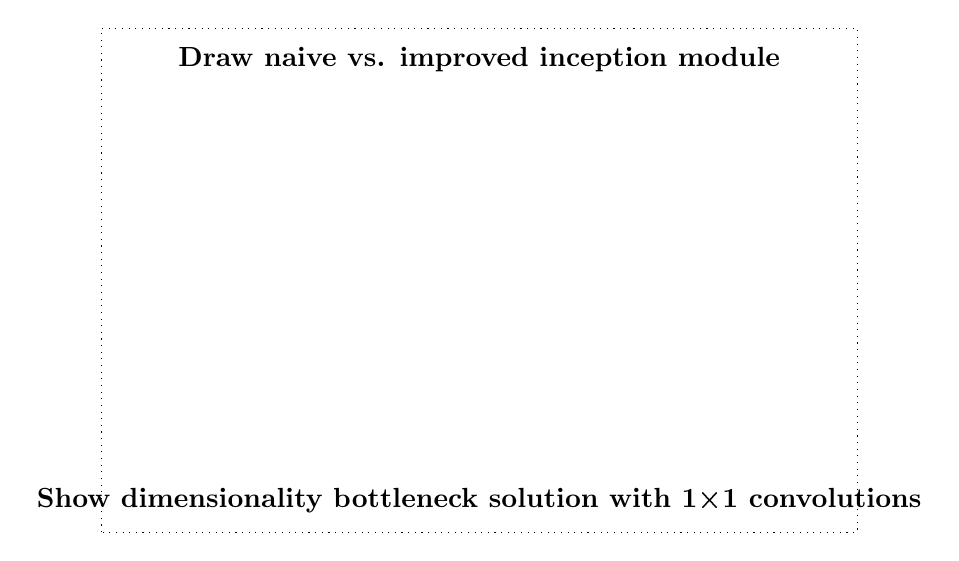
\begin{tikzpicture}[scale=0.8]
        % Space for inception module comparison
        \draw[dotted] (0,0) rectangle (12,8);
        \node at (6,7.5) {\textbf{Draw naive vs. improved inception module}};
        \node at (6,0.5) {\textbf{Show dimensionality bottleneck solution with 1×1 convolutions}};
    \end{tikzpicture}
    \end{center}
    
    \shortanswer
    
    \item Analyze GoogleNet's efficiency achievements compared to AlexNet: \hfill (8 marks)
    \begin{itemize}
        \item Parameter reduction: from 60 million (AlexNet) to 4 million (GoogleNet)
        \item Role of Global Average Pooling in reducing parameters
        \item Computational cost comparison and architectural depth (22 layers)
    \end{itemize}
    
    \mediumanswer
    
    \item Evaluate auxiliary classifiers in GoogleNet: \hfill (5 marks)
    \begin{itemize}
        \item Mathematical formulation of multi-loss training
        \item Benefits for gradient flow in deep networks
        \item Trade-offs in model generalization
    \end{itemize}
    
    \shortanswer
\end{enumerate}

\newpage
\paragraph{Question 4. ResNet and Residual Learning Theory}{\hfill (30 marks)}\\
Based on Microsoft Research ResNet paper and university deep learning theory courses.

\begin{enumerate}[(a)]
    \item Analyze the degradation problem in deep networks that ResNet addresses: \hfill (10 marks)
    \begin{itemize}
        \item Why do 56-layer CNNs perform worse than 20-layer CNNs on both training and test sets?
        \item Mathematical explanation of gradient vanishing in very deep networks
        \item Distinction between degradation problem and overfitting
    \end{itemize}
    
    \mediumanswer
    
    \item Derive the mathematical foundation of residual learning: \hfill (12 marks)
    \begin{itemize}
        \item Given target mapping $H(x)$, show why learning $F(x) = H(x) - x$ is easier than learning $H(x)$
        \item Residual block formulation: $y = F(x, \{W_i\}) + x$
        \item Gradient flow analysis: $\frac{\partial loss}{\partial x} = \frac{\partial loss}{\partial y}(1 + \frac{\partial F}{\partial x})$
        \item Explain why the "+1" term prevents gradient vanishing
    \end{itemize}
    
    \journalspace
    
    \item Compare ResNet variants and their performance characteristics: \hfill (8 marks)
    \begin{itemize}
        \item ResNet-18, ResNet-34: basic blocks vs. deeper architectures
        \item ResNet-50, ResNet-101, ResNet-152: bottleneck blocks for efficiency
        \item Performance scaling: how accuracy improves with depth up to 152 layers
        \item Computational complexity comparison with VGG architectures
    \end{itemize}
    
    \mediumanswer
\end{enumerate}

\newpage
\paragraph{Question 5. Adversarial Attacks and Defenses}{\hfill (25 marks)}\\
Based on cybersecurity research and university machine learning security courses.

\begin{enumerate}[(a)]
    \item Formulate adversarial attack optimization problems for image classification: \hfill (10 marks)
    \begin{itemize}
        \item Targeted attack: $\min_{\delta} \||\delta\||_p$ subject to $f(x + \delta) = t$ and $\||\delta\||_\infty \leq \epsilon$
        \item Untargeted attack: $\min_{\delta} \||\delta\||_p$ subject to $f(x + \delta) \neq y$ and $\||\delta\||_\infty \leq \epsilon$
        \item Explain the role of $L_p$ norms in constraint formulation
    \end{itemize}
    
    \mediumanswer
    
    \item Implement the Fast Gradient Sign Method (FGSM): \hfill (10 marks)
    \begin{itemize}
        \item Derive FGSM formula: $x' = x + \epsilon \cdot \text{sign}(\nabla_x J(\theta, x, y))$
        \item Explain why FGSM is effective against linear behavior in neural networks
        \item Calculate perturbation for a binary classification problem with cross-entropy loss
        \item Discuss computational efficiency compared to iterative methods
    \end{itemize}
    
    \mediumanswer
    
    \item Analyze defense strategies against adversarial attacks: \hfill (5 marks)
    \begin{itemize}
        \item Adversarial training: training with adversarial examples
        \item Defensive distillation: temperature-based softmax smoothing
        \item Detection methods: statistical analysis of input distributions
        \item Trade-offs between robustness and accuracy
    \end{itemize}
    
    \shortanswer
\end{enumerate}

\newpage
\paragraph{Question 6. Architecture Comparison and Evolution}{\hfill (20 marks)}\\
Based on comprehensive analysis from multiple university computer vision courses.

\begin{enumerate}[(a)]
    \item Create a comparative analysis table for CNN architectures: \hfill (12 marks)
    
    \begin{center}
    \begin{tabular}{|l|c|c|c|c|}
    \hline
    Architecture & Depth & Parameters & Top-5 Error & Key Innovation \\
    \hline
    AlexNet (2012) & 8 & 60M & 15.3\% & ? \\
    VGG-16 (2014) & 16 & 138M & ? & ? \\
    GoogleNet (2014) & 22 & 4M & ? & ? \\
    ResNet-152 (2015) & 152 & ? & ? & ? \\
    \hline
    \end{tabular}
    \end{center}
    
    Complete the table and analyze:
    \begin{itemize}
        \item Parameter efficiency trends over time
        \item Relationship between depth and performance
        \item Trade-offs between accuracy and computational cost
    \end{itemize}
    
    \mediumanswer
    
    \item Evaluate architectural design principles: \hfill (8 marks)
    \begin{itemize}
        \item Why smaller filter sizes (3×3) became preferred over larger ones (11×11, 7×7)
        \item Role of skip connections in enabling very deep networks
        \item Impact of global average pooling vs. fully connected layers
        \item Evolution from hand-crafted to learnable architectures
    \end{itemize}
    
    \shortanswer
\end{enumerate}

\newpage
\paragraph{Question 7. Feature Visualization and Interpretability}{\hfill (20 marks)}\\
Based on interpretable AI research and university courses on explainable deep learning.

\begin{enumerate}[(a)]
    \item Design feature inversion techniques for understanding CNN representations: \hfill (10 marks)
    \begin{itemize}
        \item Formulate optimization: $\min_x \||f(x) - f_0\||^2 + \lambda R(x)$
        \item Explain different regularization terms $R(x)$: total variation, $L_2$ norm
        \item Implement gradient-based optimization for feature reconstruction
        \item Analyze why early layers preserve more spatial information than later layers
    \end{itemize}
    
    \mediumanswer
    
    \item Evaluate saliency map generation methods: \hfill (10 marks)
    \begin{itemize}
        \item Vanilla gradients: $S_i = \left|\frac{\partial f_c}{\partial x_i}\right|$
        \item Integrated gradients: addressing gradient saturation problems
        \item LIME (Local Interpretable Model-agnostic Explanations): local approximation approach
        \item Quantitative evaluation metrics for explanation quality
    \end{itemize}
    
    \mediumanswer
\end{enumerate}

\vfill
\begin{center}{\bf END OF PAPER}\end{center>
\end{document>